\setcounter{page}{1}    % 将页码计数器设置为 1

% ===============================================================
%
% 问题重述与分析
%
% ===============================================================

\section{问题重述}

\subsection{问题背景}

随着互联网不断发展,线上教育平台这种新型教育模式逐渐兴起。各种基于互联网教育的模式渐渐地发展起来。利用互联网的高度便利性和自定义性,因材施教的程度得以进一步发展。为了进一步实现用户的个性化学习,某\linebreak MOOC在线教育平台提供了个性化题库的功能。该题库系统会记录用户的学习过程,并自动生成个性化的课后习题。但目前来说,该系统还存在着很大的缺陷。

为了实现自动生成个性化试题的功能,该题目系统需实现两个重要的子功能:\textbf{相似度评估系统}和\textbf{难度评估系统}。

目前而言,这两个系统都存在明显的缺陷。

\subsection{相似性评估系统}

在该系统中,度量两个题目之间的相似性主要基于\textbf{题干文字}和\textbf{题目事先标注的知识点信息}。而前者无法处理表述不同但解法类似的题目;后者则与知识点划分方式相关,难以实现真正的拓展练习。这两种方式急需改进。

\subsection{难度评估系统}

在该系统中,判断题目难度的依据主要是\textbf{考试的类型}和\textbf{教师的主观经验}。这两种方式都有较大的局限性:前者只能判断考试试题的难度,而实际上还有很多未出现在考试试题中的题目;后者过于主观,即不同的教师可能会给出截然不同的评估结果。与此同时,一个题目的难度与题面的表达、学习者的状态、学习者的知识储备等等因素有关。因此,该系统仍然需要进一步改进。

\section{问题分析}

\begin{figure}[h]
    \centering
    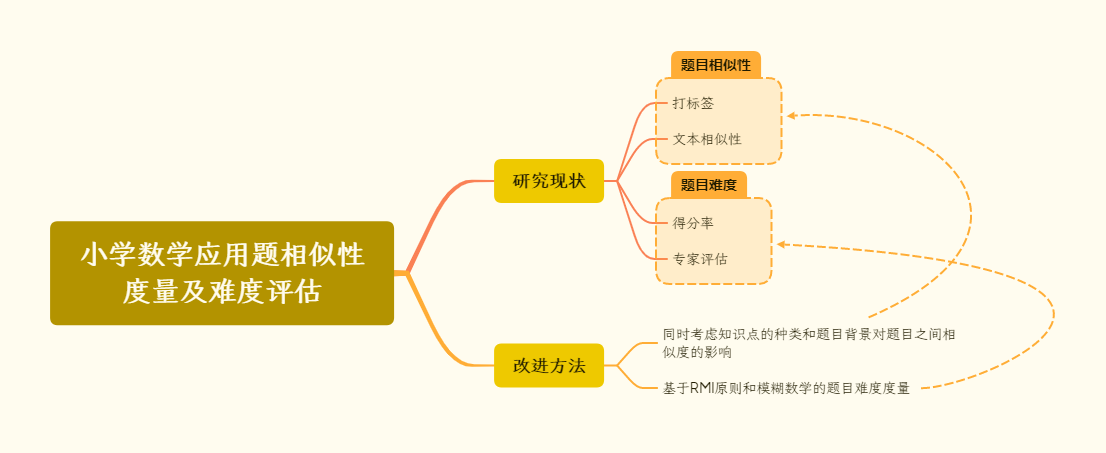
\includegraphics[scale=0.22]{res/figure042227.png}
    \caption{关于相似性度量和难度评估的改进思路}
\end{figure}
 
\subsection{关于相似性度量和难度评估的研究现状}

研究相似性度量和难度评估,可以更好地提高学生的学习效率。当今学术界对题目相似性的研究主要局限于文本的相似性。然而,这并不一定是有效的。从传统上看,有关题目相似性的研究几乎都是从打标签这一角度开始的\cite{xuTimunandupinggufangfayanjiuzongshu2022}。

当今学术界对题目相似性的研究主要局限于“打标签”。打标签是一种多维度分类的方法。这一作法,让题目之间的相似性可以局限在已有的知识体系之中。而对于题目的难度而言,目前研究的主要手段是通过得分率和教师的评分。类似这种没有将题目本身的难度和外在难度区分开来的研究占大部分。

\subsection{同时考虑知识点的种类和题目背景的相似性}

对于两个题目之间的相似性,可以从知识点种类与题目背景两个方面思考。对于题目的知识种类:两个题目所涵盖的知识种类的交集越多,这两个题目之间的相似性显然就越高;类似地,两个题目的应用背景越相似,两个题目的相似性也会越高。对于传统判断题目相似的方法,都只能考虑其中一种可能性。因此,一个更加合理的做法就是同时考虑这两个方面评估相似性。

基于以上两点思考,通过自然语言处理(Nature Language Processing, NLP)理论中的jieba中文分词系统和LDA模型处理题目,提取其内在的逻辑信息和背景信息。

这样的处理,可以较好地改善目前相似性度量系统的缺陷。

\subsection{模糊数学与题目难度评估}

对于题目的难度评估,主要从RMI原则和模糊数学两个方面分析。

\begin{figure}[h]
    \centering
    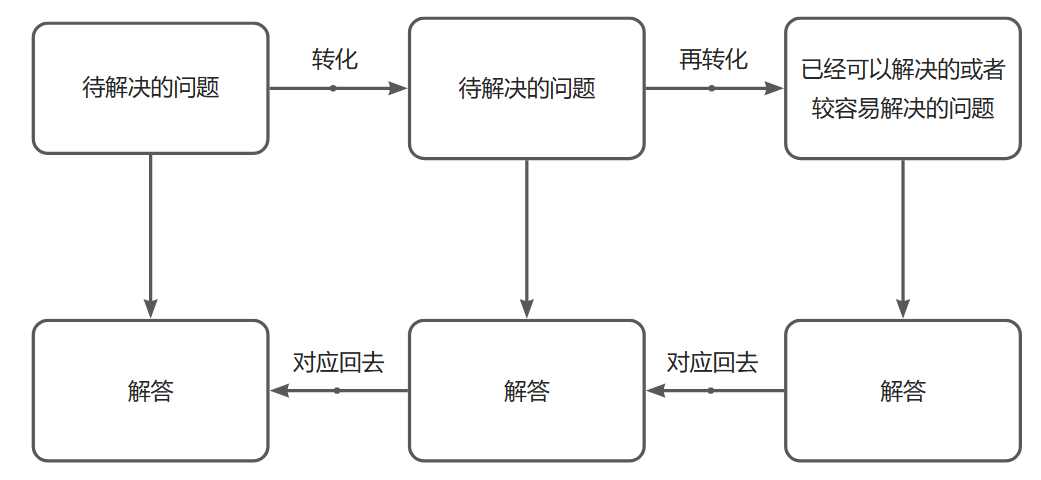
\includegraphics[scale=0.3]{res/figure040117.png}
    \caption{RMI原则}
    \label{figure040117}
\end{figure}

\paragraph{RMI原则}

RMI原则,又称关系-映射-反演(relation-mapping-inversion)原则,是由徐利治先生于上世纪80年代提出的数学方法理论\cite{zhangShuxueshitishiqiannandudeyingxiangyinsujiqilianghuayanjiu2022}。该理论认为,解决数学问题的关键在于对问题“化归”的过程。通俗来说,就是将复杂数学问题通过某种认知的方法转化为已经解决的数学问题的过程,即化繁为简。基本模式入图\ref{figure040117}所示。

\paragraph{模糊综合评价}

对于一道小学的应用题而言,决定它难度的因素除了其自身的难度外,还有许多需要避免考虑的其他因素。正如前文所言:学习者的状态和知识储备也同样会影响小学应用题的难度。在本文中,对于题目难度的评估都是对题目本身的复杂度的评估,而不考虑其他影响难度的因素。

本文主要考虑下面四个因素,其重要性依次递减:

\begin{enumerate}
    \item 知识点数量。一个题目可能包含多个知识点。所考察的知识点越多,题目难度越大。
    \item 数学运算的难易。比如解二元一次方程的难度肯定大于解一元一次方程的难度。
    \item 试题背景的复杂性。对于应用题而言,学习者需要将文字数学化。这种数学化过程的难易也会影响应用题本身的难度。
    \item 个人主观评分。有些题目具有很强技巧性。它虽然没有考察很多的知识点,也没有非常复杂的数学运算和数学背景,但是需要一种巧妙的思考才能被解出。
\end{enumerate}

\subsection{总思路}

综合以上三个小结的分析,下面给出优化题目相似性度量和题目难度评估方法的总思路(如图\ref{figure042108})。

\begin{figure}[h]
    \centering
    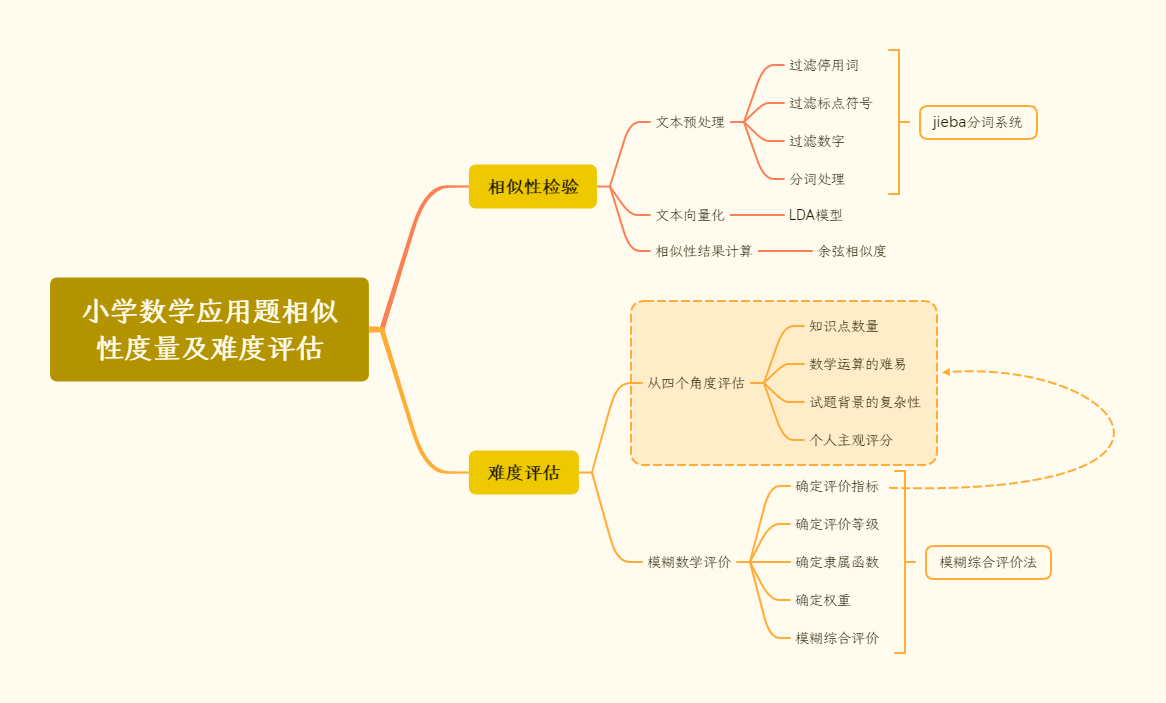
\includegraphics[scale=0.2]{res/figure042108.png}
    \caption{小学数学应用题相似性度量及难度评估的研究的总思路}
    \label{figure042108}
\end{figure}

% ===============================================================
%
% 模型假设与符号说明
%
% ===============================================================

\section{模型假设与符号说明}

\subsection{模型假设}

\begin{itemize}
    \item 假设学习者是小学教育水平;
    \item 假设每个难度评估者都是抱着尽量客观的态度进行评估作业的;
    \item 假设每道应用题都只有唯一解法;
    \item 假设题库中所考察的知识点是已知且有限的。
\end{itemize}

\subsection{符号说明}

\begin{table}[h]
    \centering
    \begin{tabular}{@{}cc@{}}
        \toprule
        \quad \quad \quad 符号 \quad \quad \quad           & 意义                       \\ \midrule
        $Z_{n,l}$     & 文档$n$中第$l$个分词对应的主题编号     \\
        $\alpha$      & 控制文档-主题分布的超参数/狄利克雷分布先验参数 \\
        $\beta$       & 控制主题-词语分布的超参数/狄利克雷分布先验参数 \\
        $w_{n,l}$     & 文档$n$中第$l$个分词对应的主题编号     \\
        $\varphi_{k}$ & 主题$k$的词汇分布               \\
        $M_{diff}$    & 题目难度矩阵                   \\
        $L_{weight}$  & 题目难度值                    \\
        $L_D$         & 题目难度系数序列                 \\
        $S_{level}$   & 难度度量等级集合                 \\ \bottomrule
    \end{tabular}
\end{table}